\question{2}{
    Defensie test de bescherming van een nieuw type scherfvest onder verschillende soorten ballistische dreiging.
    Het onderzoek vindt plaats op het militaire testterrein van de Defensie Materieel Organisatie (DMO).
    Tijdens de test worden twee munitietypen gebruikt: fragmentatiegranaten (groep $A$) en scherpschutterspatronen (groep $B$). 
    In beide gevallen wordt gebruik gemaakt van identieke scherfvesten die zijn bevestigd op testdummies.

    Per vest wordt gemeten hoe diep de kogel- of schervenimpact doordringt in de testdummy, uitgedrukt in millimeters.
    De test wordt uitgevoerd onder gecontroleerde omstandigheden (temperatuur, vocht, afstand en inslaghoek zijn constant).
    Van beide munitietypen worden acht schoten gelost op afzonderlijke vesten, waarna de penetratiediepte wordt gemeten.

    Het hoofd van de testafdeling wil weten of de scherpschutterspatronen significant dieper penetreren dan de fragmentatiegranaten.
    Bij de fragmentatiegranaten werd op basis van een steekproef van 14 metingen een gemiddelde $\overline{x_A} = 9,85$ en variantie $s_A^2 = 0,06$ gemeten.
    Bij de scherpschutterspatronen werd op basis van een steekproef van 17 metingen een gemiddelde $\overline{x_B} = 10,52$ en variantie $s_B^2 = 0,84$ gemeten.

    Voor beide populaties wordt aangenomen dat de gemiddelde hartslag normaal verdeeld is met onbekende verwachtingswaardes $\mu_A$ en $\mu_B$, en standaardafwijkingen $\sigma_A$ en $\sigma_B$.
}
    \begin{enumerate}[label=(\alph*)]
        \item Bepaal met behulp van een $F$-toets of de varianties in de penetratiediepte gelijk zijn voor fragmentatiegranaten en scherpschutterspatronen.
            Gebruik het kritieke gebied in je conclusie. 
            Kies voor het significantieniveau $\alpha = 0,03$.
        \answer{
            In de vraag staat dat we aan mogen nemen dat $X_A \sim N(\mu_A=?; \sigma_A=?)$ en $X_B \sim N(\mu_B=?; \sigma_A=?)$.

            We toetsen op gelijke varianties, oftewel de nulhypothese $H_0$ en de alternatieve hypothese $H_1$ worden als volgt gedefinieerd:
            \begin{align*}
                H_0: \quad \sigma_A^2 = \sigma_B^2 \\
                H_1: \quad \sigma_A^2 \neq \sigma_B^2
            \end{align*}

            Verder is gegeven dat we mogen werken met een significantieniveau $\alpha=0,03$, en data is al verzameld voor beide populaties.
            De toetsingsgrootheid voor een $F$-toets is gelijk aan
            \[
                F = \frac{S_A^2}{S_B^2}, 
            \]
            en volgt een $F(n-1, m-1)$-verdeling, oftewel een $F(13, 16)$-verdeling.

            De geobserveerde toetsingsgrootheid is gelijk aan
            \[
                f = \frac{s_A^2}{s_B^2} = \frac{0,06}{0,84} \approx 0,0714.
            \]
            
            Omdat we tweezijdig toetsen, is het kritieke gebied van de vorm $(-\infty; g_1]$ en $[g_2; \infty)$, waarbij de grenzen $g_1$ en $g_2$ bepaald kunnen worden met de $F(5,9)$-verdeling.
            \begin{align*}
                &\fcdf(\text{lower}=0; \text{upper}=g_1; \text{df1}=13; \text{df2}=16)=\alpha/2=0,015 \rightarrow g_1 \approx 0,2912\\
                &\fcdf(\text{lower}=g_2; \text{upper}=10^{99}; \text{df1}=13; \text{df2}=16)=\alpha/2=0,015 \rightarrow g_2 \approx 3,2041
            \end{align*}
            De berekende $f = 0,0714$ ligt dus in het kritieke gebied, dus we verwerpen de nulhypothese $H_0$.
            Er is op basis van deze steekproeven voldoende bewijs om de aanname van gelijke varianties te verwerpen.
            We mogen dus niet uitgaan van gelijke varianties.

            \begin{center}
                \resizebox{0.9\textwidth}{!}{
                    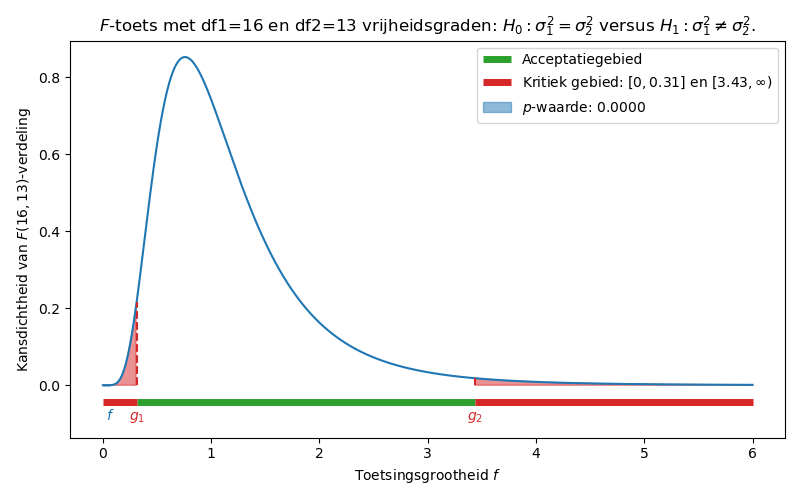
\includegraphics{oefenopgave2_Ftoets.png}
                }
            \end{center}
        }

        \item Bepaal met behulp van een onafhankelijke $t$-toets of scherpschutterspatronen gemiddeld significant dieper in een scherfvest doordringen dan fragmentatiegranaten.
            Formuleer een conclusie op basis van de $p$-waarde.
            Kies opnieuw voor het significantieniveau $\alpha = 0,03$.
        \answer{
            We toetsen of de gemiddelde penetratiediepte $\mu_B$ voor scherpschutterspatronen significant hoger is dan de gemiddelde penetratiediepte $\mu_A$ voor fragmentatiegranaten.
            De hypotheses kunnen we daarom als volgt defini\"eren:
            \begin{align*}
                H_0: \quad \mu_A \ge \mu_B \text{ (niet significant hoger) } \\
                H_1: \quad \mu_A < \mu_B \text{ (wel significant hoger) }
            \end{align*}

            Verder is gegeven dat we mogen werken met een significantieniveau $\alpha=0,03$, en data is al verzameld voor beide populaties.

            Op basis van ons antwoord bij vraag (b) moeten we aannemen dat de standaardafwijkingen $\sigma_A$ en $\sigma_B$ verschillende waardes hebben.
            Dat betekent dat we de onbekende $\sigma_A$ en $\sigma_B$ moeten schatten met respectievelijk $s_A$ en $s_B$:
                       
            De toetsingsgrootheid van de bijbehorende $t$-toets is (onder de nulhypothese $\mu_A = \mu_B$) gelijk aan
            \begin{align*}
                t &= \frac{(\overline{x_A}-\overline{x_B}) - (\mu_A - \mu_B)}{\sqrt{\frac{s_A^2}{n} + \frac{s_B^2}{m}}} \\
                  &= \frac{(9,85 - 10,52) - 0}{\sqrt{\frac{0,06}{14} + \frac{0,84}{17}}} \\
                  &\approx -2,8913, 
            \end{align*}

            en komt uit een $t$-verdeling met $\text{df}=\min(n-1, m-1) = \min(13, 16) = 13$ vrijheidsgraden.
            Omdat we linkszijdig toetsen, is de $p$-waarde gelijk aan de linkeroverschrijdingskans van de waarde $t \approx -2,8913$, oftewel
            \begin{align*}
                p = P(T \le t) = \text{tcdf}(\text{lower}=-10^{99}; \text{upper}=-2,8913; \text{df}=13) \approx 0,0063.
            \end{align*}
            
            Omdat de $p$-waarde kleiner is dan het significantieniveau $\alpha = 0,03$, moet de nulhypothese $H_0$ worden verworpen.
            Er is op basis van deze steekproeven voldoende reden om aan te nemen dat scherpschutterspatronen significant dieper doordringen dan fragmentatiegranaten.
            \begin{center}
                \resizebox{0.9\textwidth}{!}{
                    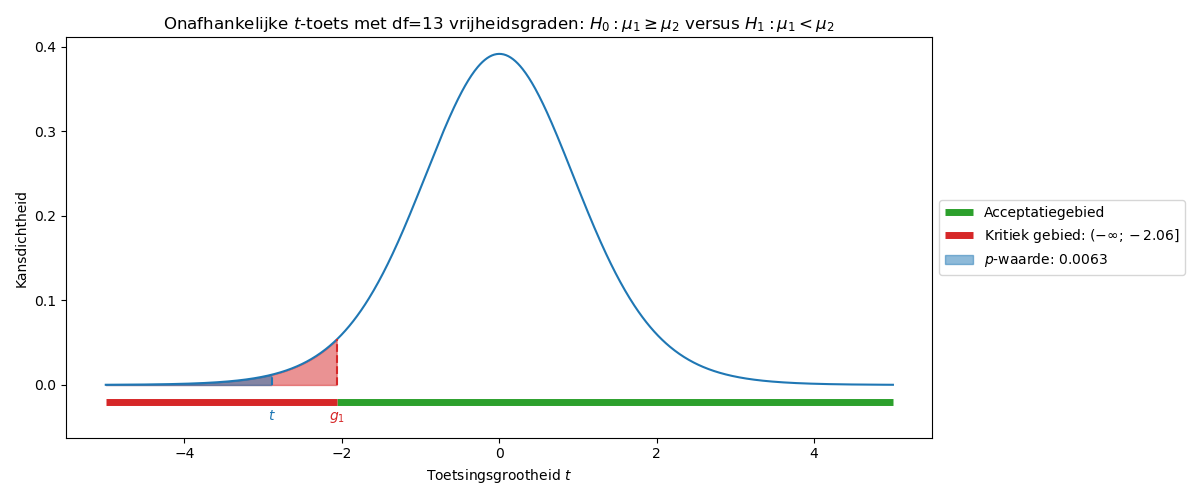
\includegraphics{oefenopgave2_ttoets.png}
                }
            \end{center}
        }    
    
    \end{enumerate}